The Higgs mechanism is the mechanism that allows the massless gauge bosons to acquire mass while preserving the $\mathrm{SU}{(2)}_{L} \otimes \mathrm{U}{(1)}_{Y}$ symmetry. To achieve this, we start by introducing a new $\mathrm{SU}(2)$ doublet of complex scalar fields,
\begin{equation}
  \phi = \begin{pmatrix}
    \phi^{+} \\
    \phi^{0}
  \end{pmatrix}
  \label{eq:higgs_doublet}
\end{equation}
where $\phi^{+}$ is a charged scalar field $\phi^{+} = \frac{1}{\sqrt{2}}(\phi_{1} + i \phi_{2})$ and $\phi^{0}$ is a neutral scalar field $\phi^{0} = \frac{1}{\sqrt{2}}(\phi_{3} + i \phi_{4})$, as well as a new term for the Standard Model Lagrangian,
\begin{equation}
  \mathcal{L}_{\mathrm{Higgs}} = {(D_{\mu}\phi)}^{\dagger}(D^{\mu}\phi) - V(\phi)
  \label{eq:higgs_lagrangian}
\end{equation}
where $D_{\mu}$ is the covariant derivative and $V(\phi)$ is known as the Higgs potential and takes the form of $V(\phi) = \mu^{2}\phi^{\dagger}\phi + \lambda{(\phi^{\dagger}\phi)}^{2}$. To extract physical masses, we can study the Higgs potential. The potential can behavior in two distinct ways depending on the sign of $\mu^{2}$:
\begin{itemize}
  \item For $\mu^{2} > 0$, the potential only has the trivial solution of $\phi = 0$, and would describe a scalar particle with mass $\mu$ and coupling $h$. 
  \item More interestingly, for $\mu^{2} < 0$ (Figure~\ref{fig:theory_higgs_potential}), the potential has a non-trivial minimum at $\phi^{0} = \sqrt{\frac{-\mu^{2}}{2\lambda}} = \frac{v}{\sqrt{2}}$, and due to the $\mathrm{U}(1)$ phase invariance, there are infinitely many of these solutions, and are referred to as the vacuum expectation value (VEV) of the Higgs field.
\end{itemize}

\begin{figure}
  \centering
  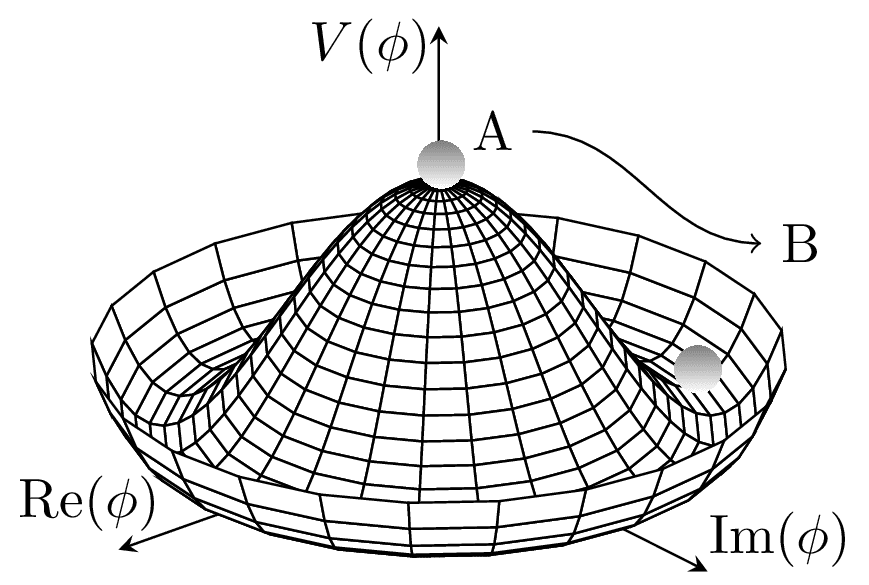
\includegraphics[width=0.5\textwidth]{figures/theory/theory_higgs_potential.png}
  \caption{The Higgs potential $V(\phi)$ as a function of the Higgs field $\phi$. The potential has a non-trivial minimum at $\phi^{0} = \sqrt{\frac{-\mu^{2}}{2\lambda}} = \frac{v}{\sqrt{2}}$ for $\mu^{2} < 0$. Taken from~\cite{riebesell_higgs_potential_2022}.}\label{fig:theory_higgs_potential}
\end{figure}

Without loss of generality, we can pick a particular vacuum solution as the ground state, thereby spontaneously breaking the original $\mathrm{SU}{(2)}_{L} \otimes \mathrm{U}{(1)}_{Y}$ symmetry down to the unbroken $\mathrm{U}{(1)}_{em}$ symmetry, which remains a true symmetry of the vacuum. To expand the Higgs field around the vacuum, we choose a specific minimum by setting $\phi_{1}=\phi_{2}=\phi_{4} = 0$ and $\phi_{3} = v$. However, there still remains fluctuations that are associated with the broken symmetry generators. These fluctuations can be parameterized by Goldstone bosons, $\theta^{i}(x)$, which appear in the field expansion as phase rotations. The expansion of the Higgs field around the VEV is
\begin{equation}
  \phi = \begin{pmatrix}
    0 \\
    \frac{v + h(x)}{\sqrt{2}}
  \end{pmatrix} e^{i\frac{\sigma_{i}}{2}\theta^{i}(x)}.
  \label{eq:higgs_expansion}
\end{equation}
We can now plug this into Equation~\ref{eq:ew_covariant_derivative} and choose the unitary gauge $\theta^{i}(x) = 0$, we see that the kinetic piece of the Lagrangian becomes
\begin{equation}
  {(D_{\mu}\phi)}^{\dagger}D^{\mu}\phi \rightarrow \frac{1}{2}\partial_{\mu}h\partial^{\mu}h + {(v+h)}^{2}\{\frac{g^{2}}{4}W_{\mu}^{\dagger}W^{\mu} + \frac{g^{2}}{8\cos^2{\theta_{W}}}Z_{\mu}Z^{\mu}   \}.
\end{equation}
The spontaneous breaking of the $\mathrm{SU}{(2)}_{L} \otimes \mathrm{U}{(1)}_{Y}$ symmetry lead to the emergence of three massless Goldstone bosons, corresponding to the three broken generators of the symmetry. The presence of these massless scalars appears to be problematic, however, by substituting the Higgs field expansion into the kinetic term of Equation~\ref{eq:higgs_lagrangian} and working in the unitary gauge, these Goldstone bosons are effectively removed. In doing so, we find that the $W^\pm$ and $Z$ bosons acquire mass, while the photon remains massless, consistent with the fact that the unbroken $\mathrm{U}(1)$ symmetry is preserved. The masses of the $W^\pm$ and $Z$ bosons are given by
\begin{align}
  m_{W} &= \frac{1}{2}g v, \\
  m_{Z} &= \frac{gv}{2\cos{\theta_{W}}}.
  \label{eq:higgs_masses}
\end{align}

With the gauge bosons now massive, we can acquire the mass terms for the fermions in a similar fashion. We can consider the fermion mass term
\begin{equation}
  \mathcal{L}_{Fermion,mass} = -m\psi\bar{\psi} = -m(\bar{\psi}_{L}\psi_{R} + \bar{\psi}_{R}\psi_{L})
\end{equation}
where $\psi$ is the fermion field. This type of mass term is not allowed due to it breaking the gauge symmetry. However, since we have introduced another scalar doublet into the model we can write a Yukawa interaction term like
\begin{equation}
  \mathcal{L}_{Yukawa} = c\bar{\psi}_{L}\phi\psi_{R} + \mathrm{h.c.}.
  \label{eq:higgs_yukawa}
\end{equation}
Using the fermion fields from Equations~\ref{eq:ew_lepton_fields} and~\ref{eq:ew_quark_fields}, we can write the Yukawa interaction term as 
\begin{equation}
  \mathcal{L}_{Yukawa} = c_{q'} {(\bar{q}, \bar{q}')}_{L}\begin{pmatrix}
    \phi^{+} \\
    \phi^{0}
  \end{pmatrix}
  q_{R}' + c_{q}{(\bar{q}, \bar{q}')}_{L}\begin{pmatrix}
    \phi^{0*} \\
    -\phi^{-}
  \end{pmatrix}
  q_{R} + c_{\ell}{(\bar{\ell}, \bar{\nu}_{\ell})_{L}}\begin{pmatrix}
    \phi^{+} \\
    \phi^{0}
  \end{pmatrix}
  \ell_{R} + h.c.
\end{equation}
where $c_{q}$, $c_{q'}$, and $c_{\ell}$ are the Yukawa couplings. After symmetry breaking and choosing the unitary gauge, the Yukawa interaction simplifies to
\begin{equation}
  \mathcal{L}_{Yukawa} = \frac{1}{\sqrt{2}}(v+h)\{c_{q'}\bar{q}'q' + c_{q}\bar{q}q + c_{\ell}\bar{\ell}\ell\}.
\end{equation}
From this, it is clear that the Standard Model does not predict the values of fermion masses since they depend on free parameters that must be determined experimentally. Additionally, it demonstrates that the fermion masses are dependent on the VEV of the Higgs field, a direct consequence of the symmetry breaking. 

The Yukawa Lagrangian assumes that each quark flavor can only transform into their corresponding `up' or `down' type quark of opposite sign. However, this assumption is not consistent with experimental observations where, for example, a $u$ quark has been found to become a $\bar{s}$ quark. This discrepancy is resolved by introducing the Cabibo-Kobayashi-Maskawa (CKM) matrix, which accounts for the fact that the weak interaction eigenstates are not the same as the mass eigenstates. The CKM matrix is a $3\times3$ unitary matrix that relates the weak interaction eigenstates to their mass eigenstates via
\begin{equation}
  \begin{pmatrix}
    d' \\
    s' \\
    b' \\
  \end{pmatrix}
  = \begin{pmatrix}
    V_{ud} & V_{us} & V_{ub} \\
    V_{cd} & V_{cs} & V_{cb} \\
    V_{td} & V_{ts} & V_{tb}
  \end{pmatrix}
  \begin{pmatrix}
    d \\
    s \\
    b \\
  \end{pmatrix}
  \label{eq:ckm_matrix}
\end{equation}
where the off-diagonal terms represent the mixing between the different quark flavors. These values are not predicted by the Standard Model and must be determined experimentally. 

We conclude by returning to the Higgs Lagrangian defined in Equation~\ref{eq:higgs_lagrangian}. After symmetry breaking and choosing the unitary gauge, the Lagrangian becomes
\begin{equation}
  \mathcal{L}_{\mathrm{Higgs}} = \frac{1}{2}\partial^{\mu}h\partial_{\mu}h - \mu^{2}h^{2} - \lambda v h^{3} - \frac{1}{4}\lambda h^{4}
\end{equation}
where the $h$ field is the Higgs boson that has mass $\sqrt{2\lambda}v$. From the Higgs Lagrangian, it is evident that the Higgs boson couples to itself through two-, three-, and four-point interaction vertices, corresponding to $hhh$ and $hhhh$ self-couplings. With this, all main ingredients of the SM Lagrangian have been introduced, we can now proceed to the Higgs boson production modes and decay channels.